\documentclass[../algebraIII_notes.tex]{subfiles}
\begin{document}
\section{Aula 14 - 28 de Maio, 2026}
\subsection{Motivações}
\begin{itemize}
	\item Adendos, comentário e exercícios sobre a aula passada;
	\item Exemplos de Uso do Teorema.
\end{itemize}
\subsection{Comentários Sobre Aula Passada}
Primeiramente, considere \(\mathbb{F}\subseteq \mathbb{M}\subseteq \mathbb{K}\) e suponha que \(\mathbb{K}/\mathbb{M}\) é Galois. É verdade que \(\mathrm{Inv}(\mathrm{Gal}(\mathbb{K}/\mathbb{M}))=\mathbb{M}\)? Ora, considere \(\mathbb{M}'=\mathrm{Inv}(\mathrm{Gal}(\mathbb{K}/\mathbb{M}))\), para o qual vale
\[
	\mathbb{M}\subseteq \mathrm{Inv}(\mathrm{Gal}(\mathbb{K}/\mathbb{M})) = \mathbb{M}'.
\]
Queremos provar o outro lado, ou seja, que \(\mathbb{M}'\) está contido em \(\mathbb{M}\). De fato,
\[
	[\mathbb{K}:\mathbb{M}'] = \mathrm{ord}(\mathrm{Gal}(\mathbb{K}/\mathbb{M}')) \leq \mathrm{ord}(\mathrm{Gal}(\mathbb{K}/\mathbb{M})) = [\mathbb{K}:\mathbb{M}].
\]
Sendo \(\mathbb{M}'= \mathrm{Inv}(\mathrm{Gal}(\mathbb{K}/\mathbb{M}'))\), obtemos:
\[
	\mathrm{Gal}(\mathbb{K}/\mathbb{M}') = \mathrm{Gal}(\mathbb{K}/\mathrm{Inv}(\mathrm{Gal}(\mathbb{K}/\mathbb{M}))) = \mathrm{Gal}(\mathbb{K}/\mathbb{M}),
\]
pois, se \(G<\mathrm{Aut}_{\mathbb{F}}(\mathbb{K})\) for finito, então
\[
	G = \mathrm{Gal}(\mathbb{K}/\mathrm{Inv}(\mathbb{G})).
\]
Logo,
\[
	[\mathbb{K}:\mathbb{M}'] = [\mathbb{K}:\mathbb{M}] \Rightarrow \mathbb{M} = \mathbb{M}'.
\]

Sobre o item 4 do teorema, o objetivo foi provar que, se \(H \trianglelefteq \mathrm{Gal}(\mathbb{K}/\mathbb{F}),\) então \(\mathrm{Inv}(H)/\mathbb{F}\) é normal. Snedo
\[
	\phi H\phi^{-1}= H, \quad \forall \phi \in \mathrm{Gal}(\mathbb{K}/\mathbb{F}),
\]
então \(\mathrm{Inv}(H)\) é \(\mathrm{Gal}(\mathbb{K}/\mathbb{F})\)-invariante, ou seja,
\[
	\phi \mathrm{Inv}(H) = \mathrm{Inv}(H).
\]
Logo, existe
\begin{align*}
	\tau : & \mathrm{Gal}(\mathbb{K}/\mathbb{F})\rightarrow \mathrm{Aut}_{\mathbb{F}}(\mathrm{Inv}(H)) \\
	       & \phi \longmapsto \phi|_{\mathrm{Inv}(H)},
\end{align*}
que é, consequentemente, um homomorfismo de grupos. O passo seguinte foi tentar entender o que é o núcleo de \(\tau \), para podermos usar o \hyperlink{isomorphism_theorem}{\textit{teorema do isomorfismo}}, que dá um subgrupo dentro de \(\mathrm{Aut}_{\mathbb{F}(\mathrm{Inv}(H))}\) isomorfo ao quociente \(\mathrm{Gal}(\mathbb{K}/\mathbb{F})/\mathrm{ker}(\tau ) \); segue que
\[
	\mathrm{ker}(T) = \{\phi \in \mathrm{Gal}(\mathbb{K}/\mathbb{F}):\; \phi (a) =a,\; \forall a\in \mathrm{Inv}(H)\} = H,
\]
ou seja, podemos usar a \hyperlink{galois_characterization}{\textit{caracterização (1) de extensões de Galois}} para obter
\[
	\mathrm{ker}(\tau ) = \mathrm{Gal}(\mathbb{K}/\mathrm{Inv}(H))=H.
\]
Com isso, ganhamos a seguinte cadeia de relações:
\begin{center}
	\begin{tikzpicture}[
			observed/.style = {rectangle, thick, text centered, draw, text width = 6em},
			latent/.style = {ellipse, thick, draw, text centered, text width = 6em},
			error/.style ={circle, thick, draw, text centered},
			confounding/.style = {rectangle, thick, text centered, draw, text width = 6em, minimum width = 5.5in},
			outcome/.style = {rectangle, thick, draw, text centered, minimum height = 3.5in, text width = 6em},
		]

		\node(T) at (-2,1){\(\mathrm{Gal}(\mathbb{K}/\mathbb{F})\)};
		\node(BL) at (-2,-2){\(\displaystyle\frac{\mathrm{Gal}(\mathbb{K}/\mathbb{F})}{H}\)};
		\node(BR) at (1,1){\(\mathrm{Im}(\tau )\)};
		\node(BR) at (4,1){\(\mathrm{Aut}_{\mathbb{F}}(\mathrm{Inv}(H))\)};

		\draw[Arrow](T)--node[midway, above] {}(BL);
		\draw[Arrow](T)--node[midway, above] {\(\tau \)}(BR);
		\draw[Arrow](BL)--node[midway, below] {}(BR);

	\end{tikzpicture}
\end{center}
Assim, se provarmos que existe um subgrupo em \(\mathrm{Aut}_{\mathbb{F}(\mathrm{Inv}(H))}\) que é igual a \(\mathbb{F}\), provamos que a extensão é de Galois, e faremos isso mostrando que \(\mathrm{Inv}(\mathrm{Im}(\tau ))=\mathbb{F}\) utilizando as \hyperlink{galois_characterization}{\textit{caracterizações (2) e (3) das extensões de Galois}}.
Como provar isso? Comece observando que
\[
	\mathrm{Inv}(\mathrm{Im}(\tau )) = \{a\in \mathrm{Inv}(H):\; \phi (a) =a,\; \forall \phi \in \mathrm{Im}(\tau )\}\supseteq \mathbb{F}.
\]
Por isso, é questão de provar a sobrejetividade de \(\tau \), que foi deixado como exercício previamente.
\subsection{Utilizando o Teorema Fundamental de Galois}
Os exemplos a seguir ilustram como utilizar o \hyperlink{fundamental_galois}{\textit{teorema fundamental teoria de Galois}} e as \hyperlink{galois_characterization}{\textit{caracterizações de extensões de Galois}}
\begin{example}[Meio fraco]
	O primeiro exemplo consiste em considerar \(\mathbb{F} = \mathbb{Q},\; \mathbb{K} = \mathbb{Q}(i)\) e \(i^{2}=-1\), tal que
	\[
		\mathbb{K} = \{a+ib:\; a, b\in \mathbb{Q}\} \Rightarrow [\mathbb{K}:\mathbb{F}]=2.
	\]
	Por isso, \(\mathbb{Q}(i)\) é um corpo de decomposição de \(f(x)=x^{2}+1\in \mathbb{F}[x]\), e, por isso, é de Galois.

	Podemos determinar a ordem do grupo de Galois a partir do grau de extensão:
	\[
		\mathrm{ord}(\mathrm{Gal}(\mathbb{K}/\mathbb{F}))=[\mathbb{K}:\mathbb{F}]=2,
	\]
	indicando que teremos dois automorfismos no grupo \(\mathrm{Gal}(\mathbb{K}/\mathbb{F});\) quais são eles?
	\[
		\mathrm{Gal}(\mathbb{K}/\mathbb{F}) = \{1, \phi \},
	\]
	onde \(\phi \) é a conjugação complexa \(\phi (i) = -i\). Logo,
	\[
		\mathrm{Gal}(\mathbb{K}/\mathbb{F})\cong \mathbb{Z}_{2}.
	\]
\end{example}
\begin{example}[Complicado]
	Vamos tomar \(\mathbb{F} = \mathbb{Q}\) e \(\mathbb{K} = \mathbb{Q}(\sqrt[]{2}, \sqrt[]{3})\); se \(f(x)=(x^{2}-2)(x^{2}-3)\in \mathbb{F}[x]\), segue que ele é redutível, mas é separável, tal que qualquer corpo de decomposição de \(f(x)\) será uma extensão de Galois sobre \(\mathbb{Q}\). Em particular, \(\mathbb{K}\) é um corpo de decomposição de \(f(x)\) sobre \(\mathbb{F}\), permitindo concluir que \(\mathbb{K}/\mathbb{F}\) é de Galois.

	Sobre o grupo de Galois, podemos ao menos determinar que
	\[
		\mathrm{ord}(\mathrm{Gal}(\mathbb{K}/\mathbb{F}))=[\mathbb{K}:\mathbb{F}].
	\]
	Por sua vez, o grau da extensão pode ser determinado observando que temos uma pequena torre de corpos da forma
	\begin{center}
		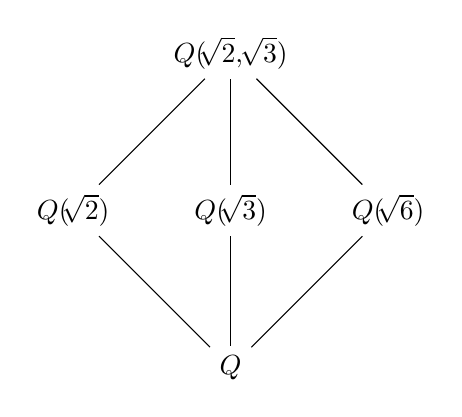
\begin{tikzpicture}[
				observed/.style = {rectangle, thick, text centered, draw, text width = 6em},
				latent/.style = {ellipse, thick, draw, text centered, text width = 6em},
				error/.style ={circle, thick, draw, text centered},
				confounding/.style = {rectangle, thick, text centered, draw, text width = 6em, minimum width = 5.5in},
				outcome/.style = {rectangle, thick, draw, text centered, minimum height = 3.5in, text width = 6em},
			]
			\node(TT) at (0,0){\(\mathbb{Q}(\sqrt[]{2}, \sqrt[]{3})\)};
			\node(TR) at (-2,-2){\(\mathbb{Q}(\sqrt[]{2})\)};
			\node(CL) at (0,-2){\(\mathbb{Q}(\sqrt[]{3})\)};
			\node(CR) at (2,-2){\(\mathbb{Q}(\sqrt[]{6})\)};
			\node(BB) at (0,-4){\(\mathbb{Q}\)};

			\draw[-](BB)--(CR);
			\draw[-](BB)--(TR);
			\draw[-](BB)--(CL);
			\draw[-](CL)--(TT);
			\draw[-](CR)--(TT);
			\draw[-](TR)--(TT);
		\end{tikzpicture}
	\end{center}
	Assim, basta demonstrar que \(p(x)=x^{2}-3\) é minimal para \(\sqrt[]{3}\) sobre \(\mathbb{Q}(\sqrt[]{2})\) [Lista de exercícios!] e concluimos que
	\[
		[\mathbb{K}:\mathbb{F}] = 4 = \mathrm{ord}(\mathrm{Gal}(\mathbb{K}/\mathbb{F})).
	\]
	Quais são estes quatro elementos?

	A ideia é mostrar que este grupo de Galois é isomorfo ao grupo de Klein:
	\[
		\mathrm{Gal}(\mathbb{K}/\mathbb{F})\cong \mathbb{Z}_2 \times \mathbb{Z}_2,
	\]
	tal que
	\[
		\mathrm{Gal}(\mathbb{K}/\mathbb{F}) = \{(\mathrm{id}, \mathrm{id}), (\mathrm{id}, \phi_1), (\mathrm{id}, \phi_2), (\phi_1, \phi_2)\},
	\]
	onde \(\phi_1\) e \(\phi_2\) são as conjugações
	\[
		\phi_1(\sqrt[]{2}) = -\sqrt[]{2} \quad\&\quad \phi_2(\sqrt[]{3})=-\sqrt[]{3}.
	\]
	De fato, \(\mathbb{Z}_2 \times \mathbb{Z}_2\) é abeliano pois todos os subgrupos são normais, e, ao todo, são 3 subgrupos:
	\[
		G_1 = \langle (\phi_1, \mathrm{id}) \rangle, \quad G_2 = \langle (\mathrm{id}, \phi_2) \rangle \quad\&\quad G_3= \langle (\phi_1, \phi_2) \rangle,
	\]
	um para cada um dos subcorpos na torre acima! Isso decorre justamente do teorema fundamental: devemos necessariamente ser capazes de associar cada um dos \(G_{i}\)'s acima com \(\mathbb{Q}(\sqrt[]{2}),\; \mathbb{Q}(\sqrt[]{3})\) e \(\mathbb{Q}(\sqrt[]{6})\), e isto é feito analisando seus invariantes.

	Primeiramente,
	\[
		\mathrm{Inv}(G_1) = \{\alpha \in \mathbb{Q}(\sqrt[]{2}, \sqrt[]{3}):\; \psi (\alpha ) = \alpha ,\; \forall \psi \in G_1\}.
	\]
	Qual é invariante a \(\phi_1\)? O grupo que não tem o \(\sqrt[]{2}\) para virar \(-\sqrt[]{2}\)! Mais explicitamente,
	\[
		\psi (a_{0}+\sqrt[]{3}a_1) = a_{0} + \psi(\sqrt[]{3})a_1 = \left\{\begin{array}{ll}
			a_{0} + \phi_1(\sqrt[]{3}) a_1 \\
			a_{0} + \mathrm{id}(\sqrt[]{3})a_1
		\end{array}\right.=a_{0}+\sqrt[]{3}a_1.
	\]
	Logo,
	\[
		\mathbb{Q}(\sqrt[]{3}) \subseteq \mathrm{Inv}(G_1) = \{\alpha \in \mathbb{Q}(\sqrt[]{2}, \sqrt[]{3}):\; \psi (\alpha ) = \alpha ,\; \forall \psi \in G_1\}.
	\]
	Por outro lado, temos a cadeia
	\[
		\mathbb{Q}\subseteq \mathbb{Q}(\sqrt[]{3})\subseteq \mathrm{Inv}(G_1)\subseteq \mathbb{Q}(\sqrt[]{2}, \sqrt[]{3}),
	\]
	e sabemos que
	\[
		[\mathbb{Q}(\sqrt[]{2}, \sqrt[]{3}):\mathbb{Q}]=4, \quad [\mathbb{Q}(\sqrt[]{2}, \sqrt[]{3}):\mathbb{Q}(\sqrt[]{3})]=2 \quad\&\quad [\mathbb{Q}(\sqrt[]{3}): \mathbb{Q}]=2.
	\]
	Com isso, ou a extensão \([\mathbb{Q}(\sqrt[]{2}, \sqrt[]{3}): \mathrm{Inv}(G_1)]=1\) e  \([\mathrm{Inv}(G_1):\mathbb{Q}(\sqrt[]{3})] = 2\), ou \([\mathrm{Inv}(G_1):\mathbb{Q}(\sqrt[]{3})] = 1\) e \([\mathbb{Q}(\sqrt[]{2}, \sqrt[]{3}): \mathrm{Inv}(G_1)]=2\).
	Como \([\mathbb{Q}(\sqrt[]{2}, \sqrt[]{3}): \mathrm{Inv}(G_1)]\neq 1\) porque já sabemos que são diferentes, resta apenas a conclusão de que \([\mathrm{Inv}(G_1):\mathbb{Q}(\sqrt[]{3})] = 1\), e que portanto
	\[
		\mathrm{Inv}(G_1) = \mathbb{Q}(\sqrt[]{3}).
	\]

	O mesmo raciocínio mostra que
	\[
		\mathrm{Inv}(G_2) = \mathbb{Q}(\sqrt[]{2}) \quad\&\quad \mathrm{Inv}(G_3) = \mathbb{Q}(\sqrt[]{6}).
	\]
\end{example}

\begin{example}[Mais Complicado]
	Desta vez, vamos considerar \(\mathbb{F} = \mathbb{Q}\) e \(f(x)=x^{3}-2\in \mathbb{F}[x]\); queremos \textbf{encontrar um corpo de decomposição} de \(f(x)\) sobre \(\mathbb{F}\), e, uma vez que tenhamos ele, procuraremos uma extensão normal finita, que será de Galois.
	Observe que, se fizermos \(f'(x)\), obtemos
	\[
		f'(x) = 3x^{2} \Rightarrow \mathrm{mdc}(f(x), f'(x))=1,
	\]
	tal que \(f(x)\) é separável. O próximo passo natural é \textbf{buscar as raízes de f}:
	\[
		\alpha_1 = \sqrt[3]{2}, \quad \alpha_2 = \sqrt[3]{2}\biggl(\frac{-1+\sqrt[]{-3}}{2}\biggr) \quad\&\quad \alpha_3 = \sqrt[3]{2}\biggl(\frac{-1-\sqrt[]{-3}}{2}\biggr),
	\]
	obtidas resolvendo o polinômio quadrático obtido ao fatorar \(x-\sqrt[3]{2}\)
	\[
		x^{3}-2 = (x-\sqrt[3]{2})(x^{2}+\sqrt[3]{2}x + \sqrt[3]{4}).
	\]
	Um corpo de decomposição de \(f(x)\) é, então, \(\mathbb{K} = \mathbb{Q}(\sqrt[3]{2}, \sqrt[]{-3})\)

	Tendo conhecimento do corpo de decomposição, precisamos \textbf{determinar o grau da extensão}, que pode ser feito escolhendo um caminho na torre (não contém todos os subcorpos possíveis!)
	\begin{center}
		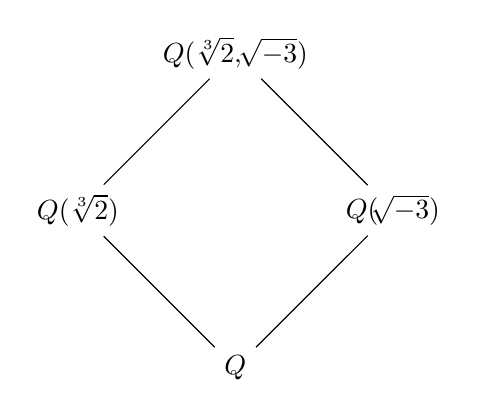
\begin{tikzpicture}[
				observed/.style = {rectangle, thick, text centered, draw, text width = 6em},
				latent/.style = {ellipse, thick, draw, text centered, text width = 6em},
				error/.style ={circle, thick, draw, text centered},
				confounding/.style = {rectangle, thick, text centered, draw, text width = 6em, minimum width = 5.5in},
				outcome/.style = {rectangle, thick, draw, text centered, minimum height = 3.5in, text width = 6em},
			]
			\node(TT) at (0,0){\(\mathbb{Q}(\sqrt[3]{2}, \sqrt[]{-3})\)};
			\node(TR) at (-2,-2){\(\mathbb{Q}(\sqrt[3]{2})\)};
			\node(CR) at (2,-2){\(\mathbb{Q}(\sqrt[]{-3})\)};
			\node(BB) at (0,-4){\(\mathbb{Q}\)};

			\draw[-](BB)--(CR);
			\draw[-](BB)--(TR);
			\draw[-](CR)--(TT);
			\draw[-](TR)--(TT);
		\end{tikzpicture}
	\end{center}
	Pela direita, o polinômio minimal é \(p(x) = x^{2}+3\), e, pela esquerda, é \(f(x)=x^{3}-2\); logo, pelo mesmo raciocínio de antes,
	\[
		[\mathbb{Q}(\sqrt[3]{2}, \sqrt[]{-3}):\mathbb{Q}]=[\mathbb{Q}(\sqrt[3]{2}):\mathbb{Q}(\sqrt[3]{2})][\mathbb{Q}(\sqrt[3]{2}):\mathbb{Q}]=3 \times 2 = 6,
	\]
	tal que
	\[
		\mathrm{ord}(\mathrm{Gal}(\mathbb{Q}(\sqrt[3]{2}, \sqrt[]{-3})/\mathbb{Q}))=6.
	\]

	Será que conseguimos \textbf{dar uma cara aos elementos do grupo de Galois}? Neste caso, queremos provar que \(\mathrm{Gal}(\mathbb{Q}(\sqrt[3]{2}, \sqrt[]{-3})/\mathbb{Q})\cong S_{3}\), e um argumento que podemos usar é mostrar que existe um isomorfismo:
	\begin{align*}
		\Lambda : & \mathrm{Gal}(\mathbb{Q}(\sqrt[3]{2}, \sqrt[]{-3})/\mathbb{Q})\rightarrow S_{3} \\
		          & \phi \longmapsto  \sigma_{\phi },
	\end{align*}
	onde
	\[
		\phi (\alpha_{i}) = \alpha_{\sigma_{\phi }(i)}
	\]
	é a ordenação/permutação das raízes por \(\sigma_{\phi }\), de modo que \(\Lambda(\varphi ) = \sigma_{\varphi }\).

	Temos que mostrar que este \(\Lambda \) é um homomorfismo injetor, pois isto dá o isomorfismo que queríamos. Com efeito, para ver que \(\Lambda \) é um homomorfismo de grupos, note que
	\[
		\Lambda (\varphi \psi ) = \sigma_{\varphi \psi },
	\]
	e
	\begin{align*}
		(\varphi \psi )(\alpha_{i}) = \varphi (\psi (\alpha_{i})) & = \varphi(\alpha_{\sigma_{\psi }(i)})           \\
		                                                          & = \alpha_{\sigma_{\varphi }(\sigma_{\psi }(i))} \\
		                                                          & = \alpha_{\sigma_{\psi }(\sigma_{\varphi }(i))} \\
		                                                          & =(\psi \varphi )(\alpha_{i}).
	\end{align*}
	Logo, para todos \(\varphi , \psi\),
	\[
		\Lambda (\varphi \psi ) = \Lambda (\psi \varphi ).
	\]
	Ademais,
	\[
		\Lambda (\mathrm{id}) = \sigma_{\mathrm{id}} = \mathrm{id}_{S_{3}},
	\]
	restando apenas mostrar a injetividade. De fato,
	\[
		\mathrm{ker}(\Lambda ) = \{\varphi \in \mathrm{Gal}(\mathbb{K}/\mathbb{F}):\; \Lambda (\varphi ) = \mathrm{id}_{S_{3}}\},
	\]
	mas
	\[
		\Lambda (\varphi ) = \sigma_{\varphi } = \mathrm{id}\in S_{3}\Longleftrightarrow \sigma_{\varphi }(i) = i, \quad i=1, 2, 3.
	\]
	Assim, se \(\varphi \) for um elemento no núcleo de \(\Lambda \), vale
	\[
		\varphi (\alpha_{i})=\alpha_{\sigma_{\varphi }(i)} = \alpha_{i} \Rightarrow \varphi\in \mathrm{ker}\Lambda \Longleftrightarrow \varphi(\alpha_{i})=\alpha_{i},
	\]
	ou seja, \(\mathrm{ker}(\Lambda ) = \{\mathrm{id}\}\). Como os dois grupos têm a mesma ordem e existe um homomorfismo injetor entre eles, vale \(\Lambda \) é um isomorfismo entre os grupos.

	Agora que temos essa informação, podemos tentar analisar um pouco essa extensão pelo ponto de vista do \hyperlink{fundamental_galois}{\textit{teorema fundamental}}, considerando todos os subgrupos de \(S_{3}\) para obter as subextensões. Como essa correspondência é injetora, encontrar todos os subgrupo leva a todas as subextensões!
	Vamos procurar os subgrupos de \(S_{3}\): primeiramente, \(S_{3} \) é um grupo de ordem 3, tal que seus subgrupos têm ou ordem 3, ou ordem 2, e com a notação de ciclos, caracteriza-se \(S_{3}\) pelas permutações:
	\[
		S_{3} = \{\mathrm{id}, \underbrace{(12), (13), (23)}_{\text{ordem 2}}, \underbrace{(123), (132)}_{\text{ordem 3}}\}.
	\]
	Logo, temos 3 elementos de ordem 2 que gerarão 3 subgrupos de ordem 2, e 2 elementos de ordem 3 que gerarão 2 subgrupos de ordem 3; apesar dos elementos serem distintos, \((123)^{2}=(132)\), tal que eles geram o mesmo subgrupo:
	\[
		\langle (123) \rangle = \langle (132) \rangle = A_{3},
	\]
	que é o grupo alternado de 3 elementos. Cada um dos subgrupos de ordem 2 gerados pelos elementos não é normal (exercício), e a situação aqui é a seguinte:
	\begin{center}
		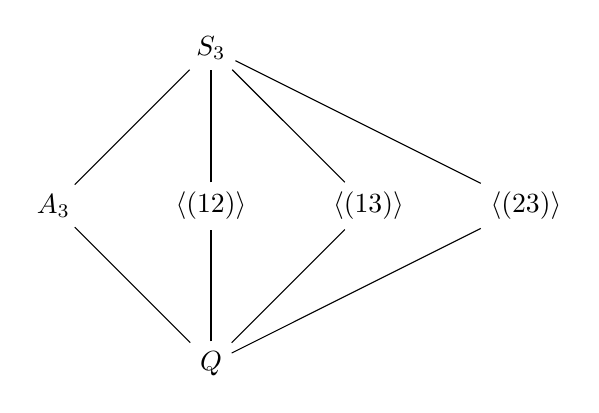
\begin{tikzpicture}[
				observed/.style = {rectangle, thick, text centered, draw, text width = 6em},
				latent/.style = {ellipse, thick, draw, text centered, text width = 6em},
				error/.style ={circle, thick, draw, text centered},
				confounding/.style = {rectangle, thick, text centered, draw, text width = 6em, minimum width = 5.5in},
				outcome/.style = {rectangle, thick, draw, text centered, minimum height = 3.5in, text width = 6em},
			]
			\node(TT) at (0,0){\(S_3\)};
			\node(TR) at (-2,-2){\(A_3\)};
			\node(CL) at (0,-2){\(\langle (12) \rangle\)};
			\node(CR) at (2,-2){\(\langle (13) \rangle\)};
			\node(CRR) at (4,-2){\(\langle (23) \rangle\)};
			\node(BB) at (0,-4){\(\mathbb{Q}\)};

			\draw[-](BB)--(CR);
			\draw[-](BB)--(CRR);
			\draw[-](BB)--(TR);
			\draw[-](BB)--(CL);
			\draw[-](CL)--(TT);
			\draw[-](CR)--(TT);
			\draw[-](CRR)--(TT);
			\draw[-](TR)--(TT);
		\end{tikzpicture}
	\end{center}
	A partir disso, as subextensões de \(\mathbb{K}/\mathbb{F}\) serão o \(\mathrm{Inv}(\cdot )\) para cada um dos subgrupos.
\end{example}
\end{document}
